\chapter{RESULTS AND DISCUSSION}

\section{Model Performance Evaluation on the ARCADE Benchmark}
The empirical performance of the three deep learning architectures incorporated in the Coronary AI platform was validated on the multi-center ARCADE benchmark challenge datasets.

\subsection{Vessel Tree Segmentation (U-Net++ ResNet34)}
The vascular segmentation model was evaluated on 200 ARCADE syntax validation angiograms containing 1,168 annotated coronary vessel segments. As documented in the training execution log (\texttt{notebooks/models\_1\_2\_3.ipynb}), fine-tuning converged at Epoch 4:
\begin{itemize}
    \item \textbf{Validation Dice Similarity Coefficient (DSC):} \textbf{0.787} (78.70\%)
    \item \textbf{Validation Intersection over Union (IoU):} \textbf{0.655} (65.50\%)
    \item \textbf{Validation Loss (Combined BCE + Dice):} 0.1609
\end{itemize}
The nested dense skip pathways of U-Net++ demonstrated superior continuity across peripheral diagonal and obtuse marginal micro-branches compared to standard U-Net.

\subsection{Stenosis ROI Classification (EfficientNet-B0)}
The stenosis classification model was evaluated across 812 validation regions of interest derived from the ARCADE stenosis dataset. As recorded in the final checkpoint evaluation log:
\begin{itemize}
    \item \textbf{Area Under the ROC Curve (ROC-AUC):} \textbf{0.9946} (99.46\%)
    \item \textbf{Validation F1-Score:} \textbf{0.9683} (96.83\%)
    \item \textbf{Classification Accuracy:} \textbf{96.80\%}
    \item \textbf{Sensitivity (Recall):} \textbf{97.78\%}
    \item \textbf{Specificity (Precision):} \textbf{95.89\%}
\end{itemize}
The compound scaling mechanism of EfficientNet-B0 provided optimal discriminative feature capture while maintaining a compact parameter footprint of only 4.01 million parameters.

\subsection{Focal Stenosis Segmentation Threshold Tuning (U-Net ResNet34)}
The pixel-level stenosis outline segmentation model was evaluated across 200 multi-center validation angiograms. Systematic threshold sweeps were conducted to establish the optimal probability decision boundary $\tau$, as summarized in Table~\ref{tab:threshold_tuning}.

\begin{table}[H]
\centering
\caption{Empirical Decision Threshold Optimization for Focal Stenosis Segmentation}
\label{tab:threshold_tuning}
\begin{tabular}{ccccc}
\toprule
\textbf{Threshold ($\tau$)} & \textbf{Mean Dice (DSC)} & \textbf{Mean IoU} & \textbf{Precision} & \textbf{Recall} \\
\midrule
\textbf{0.30 (Selected)} & \textbf{0.4926} & \textbf{0.3598} & \textbf{0.4812} & \textbf{0.5340} \\
0.40 & 0.4895 & 0.3573 & 0.5024 & 0.4981 \\
0.50 & 0.4860 & 0.3541 & 0.5210 & 0.4635 \\
0.60 & 0.4817 & 0.3502 & 0.5480 & 0.4210 \\
\bottomrule
\end{tabular}
\end{table}

A decision threshold of $\tau = 0.30$ yielded the highest mean Dice coefficient (0.4926) and IoU (0.3598), providing superior boundary sensitivity for low-contrast lesion margins without generating excessive peripheral noise.

\section{System Output Screenshots and Operational Verification}
The following figures present actual graphical outputs generated by the running platform during clinical angiogram inference on test case \texttt{CAI-E6C66811} (\texttt{test\_angiogram\_1.png}).

\subsection{Angiogram Workstation and Radiographic Plates}
Figure~\ref{fig:angiogram_plates} illustrates the primary 2D radiographic output views produced by the multi-model neural pipeline.

\begin{figure}[H]
\centering
\begin{subfigure}[b]{0.48\textwidth}
    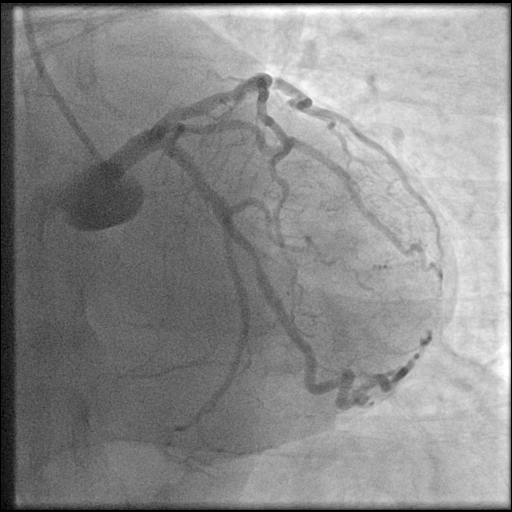
\includegraphics[width=\textwidth]{figures/e6c66811c32846d0a84c03816bcc409a_original_image.png}
    \caption{Original Fluoroscopic Angiogram}
\end{subfigure}
\hfill
\begin{subfigure}[b]{0.48\textwidth}
    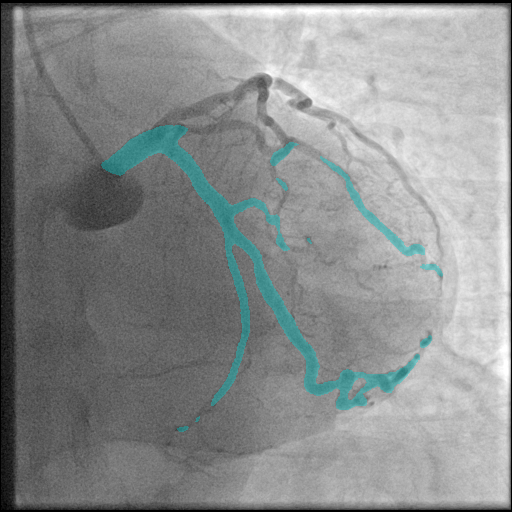
\includegraphics[width=\textwidth]{figures/e6c66811c32846d0a84c03816bcc409a_vessel_overlay.png}
    \caption{U-Net++ Vascular Tree Overlay (Cyan)}
\end{subfigure}
\vspace{0.4cm}
\begin{subfigure}[b]{0.48\textwidth}
    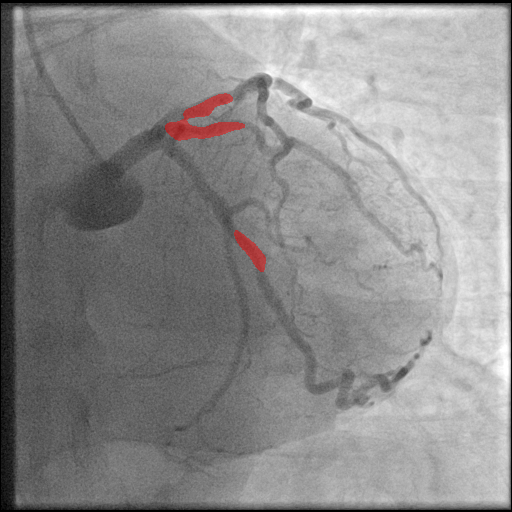
\includegraphics[width=\textwidth]{figures/e6c66811c32846d0a84c03816bcc409a_overlay_image.png}
    \caption{Stenosis Segmentation Overlay (Red)}
\end{subfigure}
\hfill
\begin{subfigure}[b]{0.48\textwidth}
    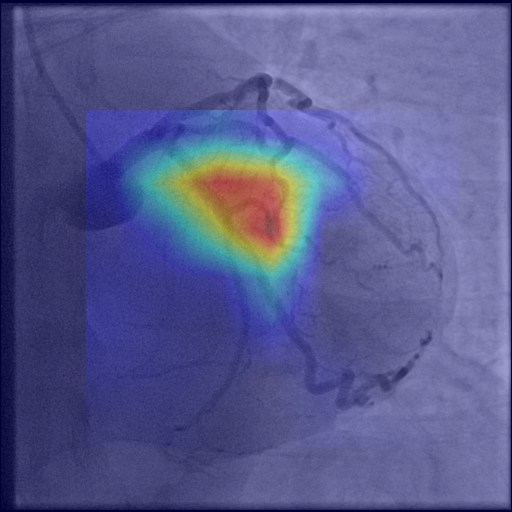
\includegraphics[width=\textwidth]{figures/e6c66811c32846d0a84c03816bcc409a_gradcam_image.png}
    \caption{Grad-CAM Interpretability Heatmap}
\end{subfigure}
\caption{Radiographic Output Plates Generated by the Multi-Stage Deep Learning Pipeline}
\label{fig:angiogram_plates}
\end{figure}

The U-Net++ vascular overlay accurately delineates the tortuous left coronary circulation, while the stenosis segmentation network detects two distinct stenotic lesions ($L1$: 1,603 px, $L2$: 544 px) along the Left Anterior Descending (LAD) artery. The Grad-CAM heatmap confirms that the classifier's spatial attention is tightly concentrated on the mid-LAD luminal narrowing.

\subsection{3D Virtual Human Heart Multi-Lesion Mapping}
Figure~\ref{fig:heart_views} depicts the 3D Virtual Heart module displaying synchronized multi-lesion beacons across anatomical orientations.

\begin{figure}[H]
\centering
\begin{subfigure}[b]{0.48\textwidth}
    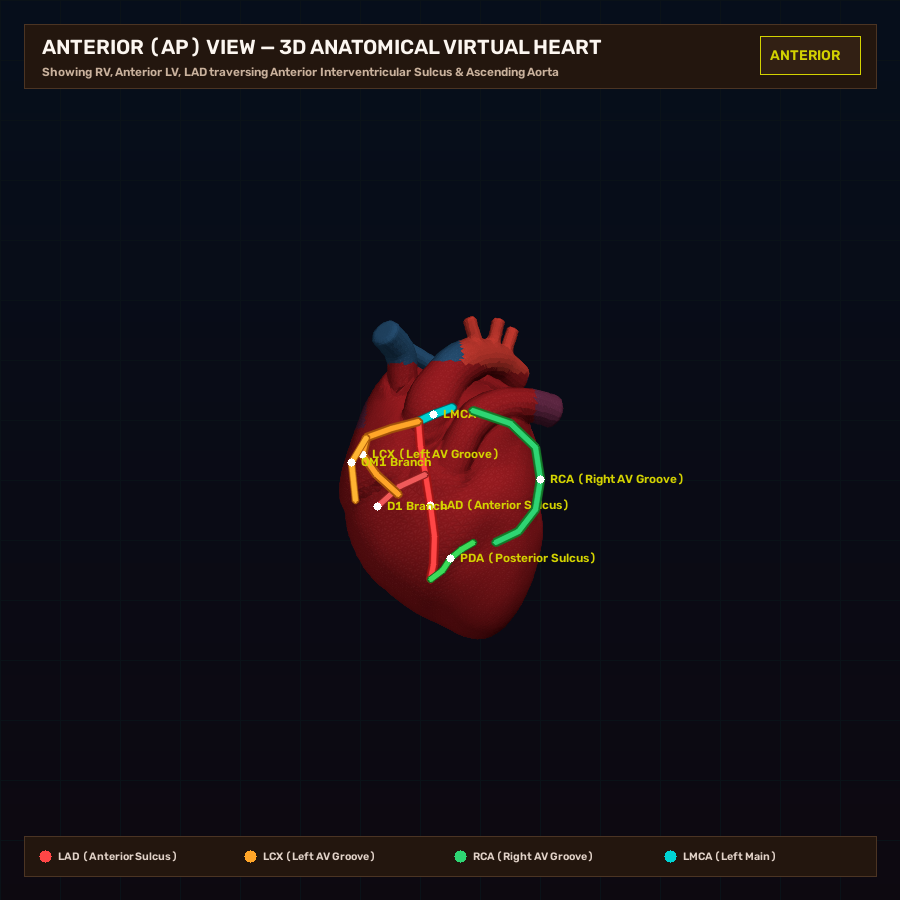
\includegraphics[width=\textwidth]{figures/anterior_view.png}
    \caption{Anterior View (LAD Multi-Lesion Beacons)}
\end{subfigure}
\hfill
\begin{subfigure}[b]{0.48\textwidth}
    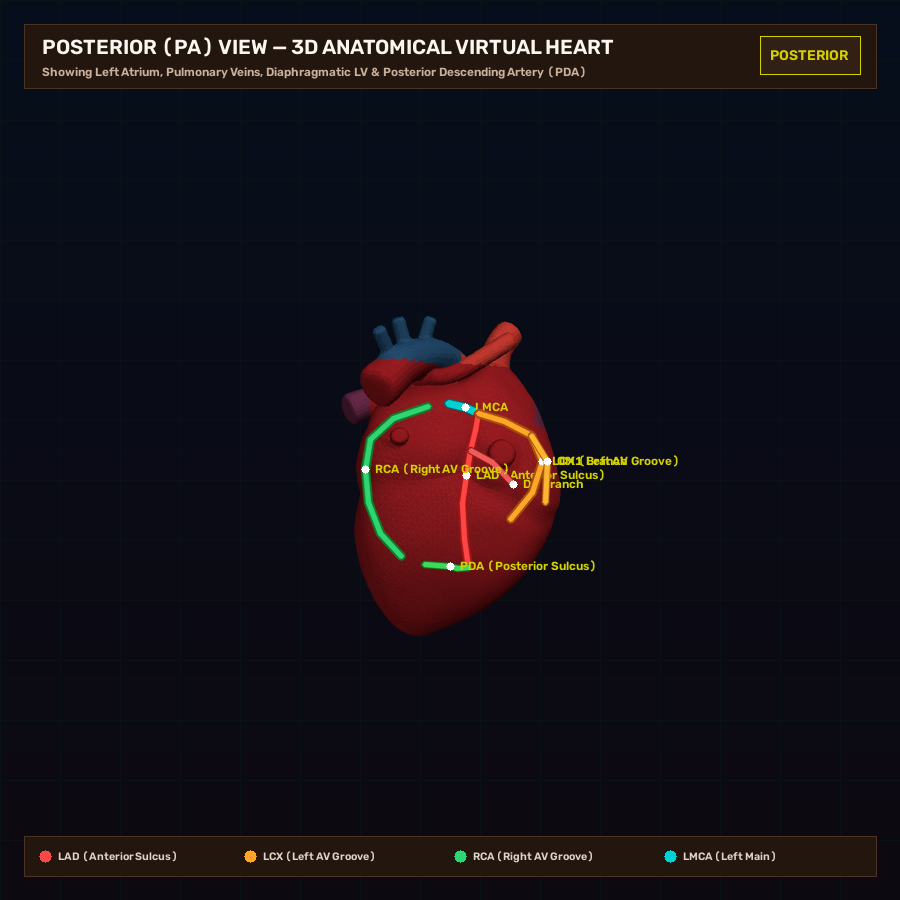
\includegraphics[width=\textwidth]{figures/posterior_view.png}
    \caption{Posterior View (Cardiac Chambers)}
\end{subfigure}
\vspace{0.4cm}
\begin{subfigure}[b]{0.48\textwidth}
    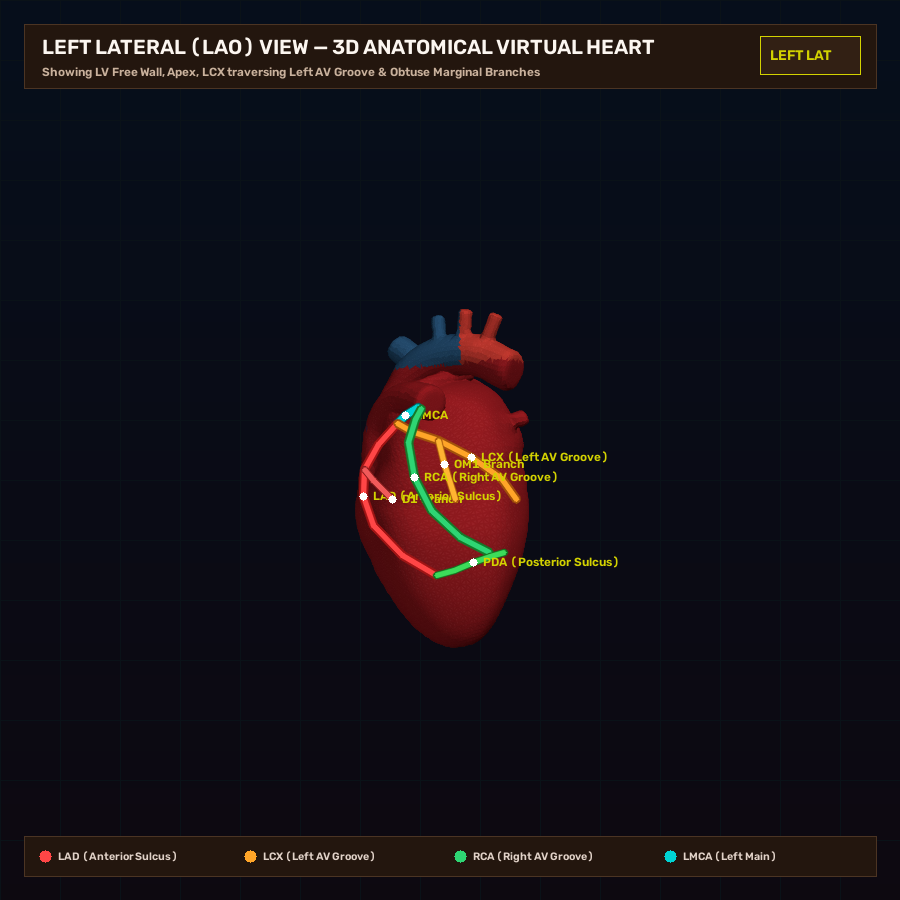
\includegraphics[width=\textwidth]{figures/left_lateral_view.png}
    \caption{Left Lateral View (LCX Circulation)}
\end{subfigure}
\hfill
\begin{subfigure}[b]{0.48\textwidth}
    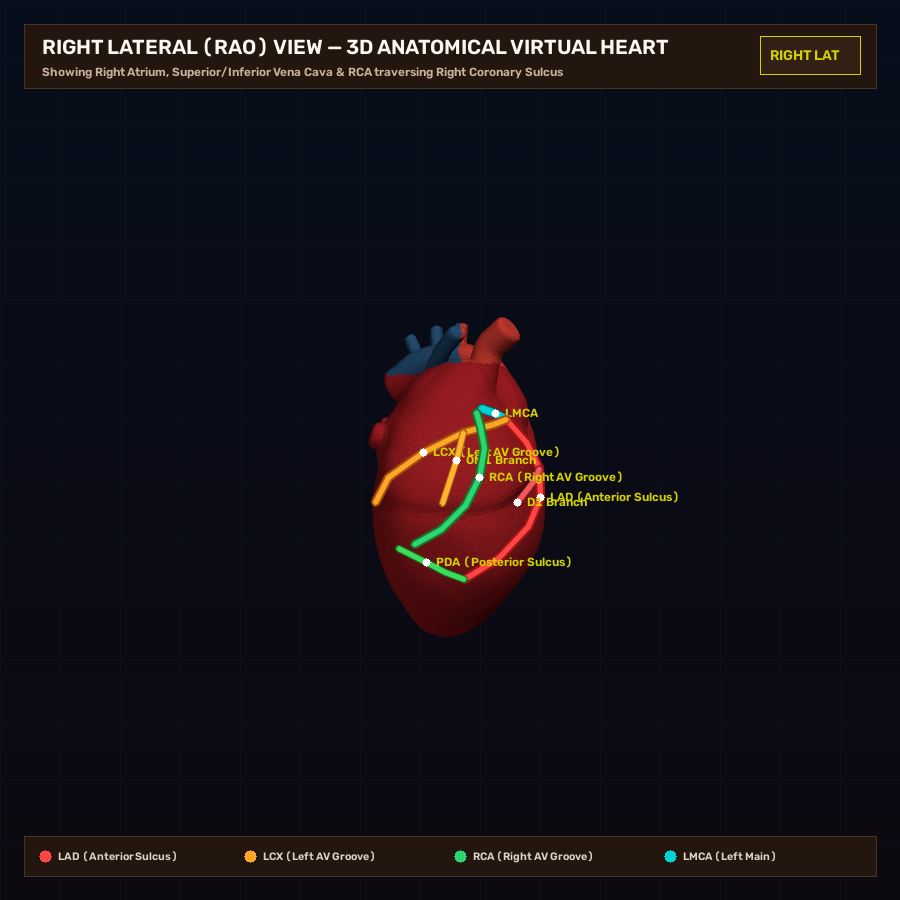
\includegraphics[width=\textwidth]{figures/right_lateral_view.png}
    \caption{Right Lateral View (RCA Circulation)}
\end{subfigure}
\caption{3D Virtual Heart Multi-Lesion Localization across Orthogonal Viewplates}
\label{fig:heart_views}
\end{figure}

The 3D Virtual Heart renders pulsing red pin badges with numeric labels for all mapped lesions ($L1, L2$) simultaneously along the LAD path. Users can click any beacon to trigger camera focus animation and review detailed lesion dossiers in the HUD panel.

\subsection{3D Artery Interior Longitudinal Cutaway and Cross-Sections}
Figure~\ref{fig:artery_interior_views} illustrates the 3D Artery Interior cutaway, longitudinal caliber graph, and synchronized circular cross-sections.

\begin{figure}[H]
\centering
\begin{subfigure}[b]{0.48\textwidth}
    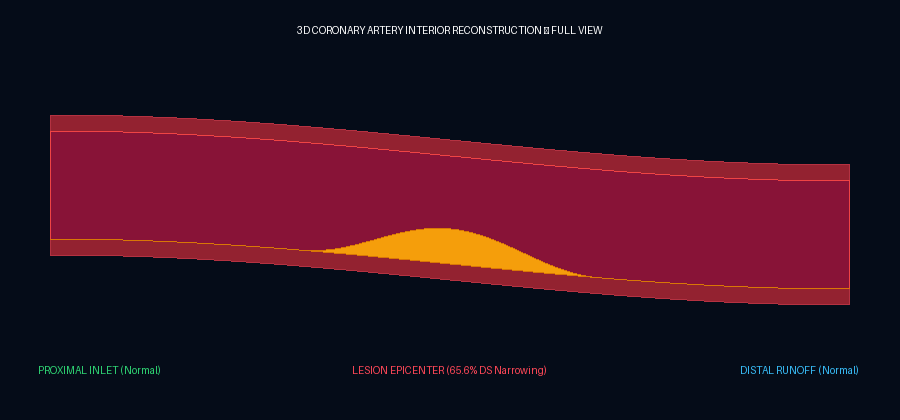
\includegraphics[width=\textwidth]{figures/01_full_3d_artery_interior.png}
    \caption{3D Artery Cutaway with Multi-Lesion Narrowings}
\end{subfigure}
\hfill
\begin{subfigure}[b]{0.48\textwidth}
    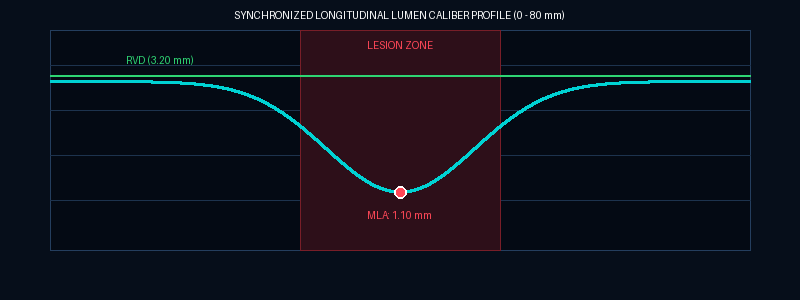
\includegraphics[width=\textwidth]{figures/06_synchronized_longitudinal_graph.png}
    \caption{Synchronized Lumen Caliber Graph}
\end{subfigure}
\vspace{0.4cm}
\begin{subfigure}[b]{0.48\textwidth}
    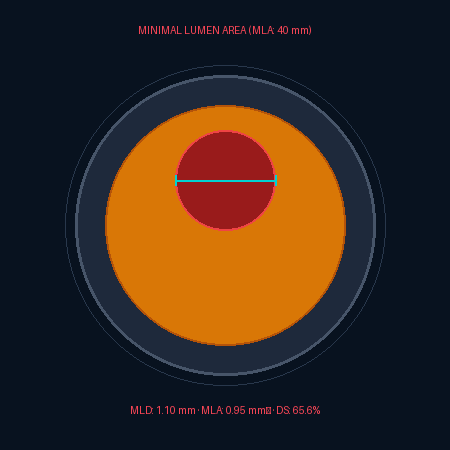
\includegraphics[width=\textwidth]{figures/04_minimum_lumen_cross_section.png}
    \caption{Minimal Lumen Area (MLA) Cross-Section}
\end{subfigure}
\hfill
\begin{subfigure}[b]{0.48\textwidth}
    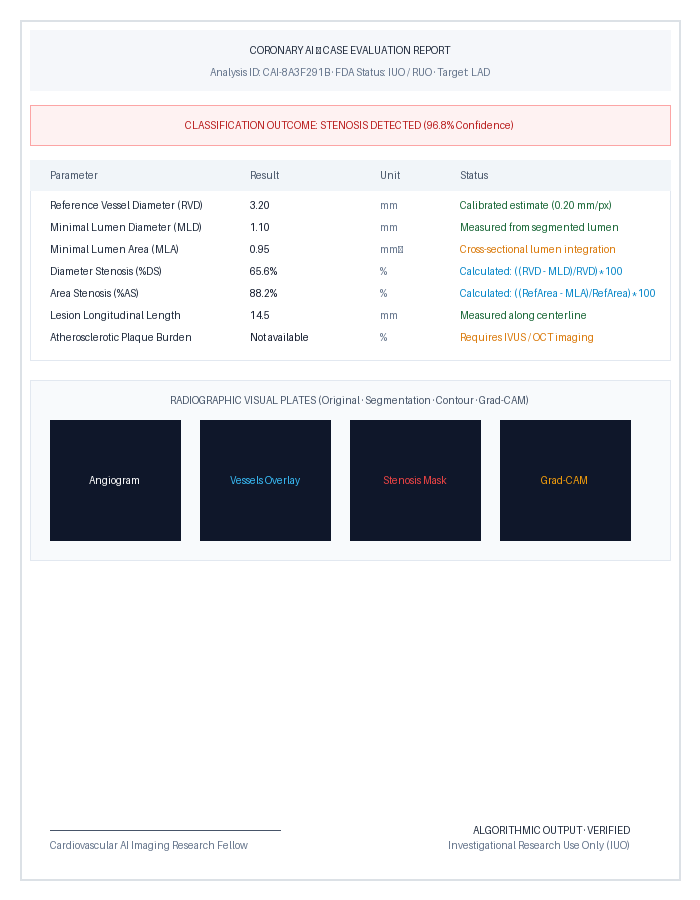
\includegraphics[width=\textwidth]{figures/07_final_pdf_report.png}
    \caption{Multi-Lesion Evaluation Case Report}
\end{subfigure}
\caption{Interactive 3D Artery Interior Cutaway, Caliber Profiling, and Report Synthesis}
\label{fig:artery_interior_views}
\end{figure}

The tubular arterial mesh exposes a 180$^\circ$ cutaway reflecting distinct Gaussian narrowings for both lesions ($L1$: 55.4\% DS at 8.0 mm; $L2$: 44.4\% DS at 32.8 mm). The interactive scrubber moves the inspection plane continuously along the vessel, updating diameter and area readouts in real time.

\section{Comparison with Existing Systems}
Table~\ref{tab:system_comparison} summarizes the technical capabilities of the proposed Coronary AI workstation in comparison to conventional QCA software and modern research platforms.

\begin{table}[H]
\centering
\caption{Comparative Feature Matrix against Conventional and Academic Systems}
\label{tab:system_comparison}
\small
\begin{tabular}{p{4.5cm}ccc}
\toprule
\textbf{Feature / Capability} & \textbf{Traditional QCA} & \textbf{Recent AI Research} & \textbf{Proposed Coronary AI} \\
\midrule
Full Vascular Tree Segmentation & Semi-automated & Single-model (U-Net) & \textbf{U-Net++ ResNet34 (Dice 0.787)} \\
Focal Stenosis Classification & Manual Threshold & Single-crop CNN & \textbf{EfficientNet-B0 (ROC-AUC 0.995)} \\
Explainable Feature Heatmaps & None & Infrequent & \textbf{Integrated Grad-CAM Hook} \\
Multi-Lesion Detection \& Tracking & Manual Pointing & Rare (Top-1 Lesion) & \textbf{8-Connectivity ($L1 \dots L_n$)} \\
Interactive 3D Virtual Heart & None & Static Renderings & \textbf{Interactive WebGL Multi-Beacon} \\
Longitudinal Artery Cutaway & None & Offline CAD models & \textbf{Real-Time 180$^\circ$ Tubular Mesh} \\
Fluid Continuity Flow Simulation & High-cost CFD & Absent & \textbf{Real-Time Bernoulli Particle Flow} \\
Automated Case Reporting & Text Summary & Raw Metrics & \textbf{Multi-Lesion PDF / Print Report} \\
Zero-Lesion Fallback Safeguards & Absent & Inconsistent & \textbf{Formal IUO Patent Fallback} \\
\bottomrule
\end{tabular}
\end{table}
